\documentclass[DIN, pagenumber=false, fontsize=11pt, parskip=half]{scrartcl}
\usepackage[UTF8]{ctex}  % 中文支持
% \usepackage{ngerman}
\usepackage[utf8]{inputenc}
\usepackage[T1]{fontenc}
\usepackage{textcomp}
\usepackage{graphicx}
\usepackage{amsmath}
\usepackage{booktabs}

\usepackage{xcolor} % Required for custom red

\usepackage{geometry} % Custom margins

\usepackage{tocloft} % Modifying the table of contents

% for matlab code
% bw = blackwhite - optimized for print, otherwise source is colored
\usepackage[framed,numbered,bw]{mcode}
\usepackage[most]{tcolorbox}
% for other code
%\usepackage{listings}

\setlength{\parindent}{0em}

% set section in CM
\setkomafont{section}{\normalfont\bfseries\Large}

\newcommand{\mytitle}[1]{{\noindent\Large\textbf{#1}}}
\newcommand{\mysection}[1]{\textbf{\section*{#1}}}
\newcommand{\mysubsection}[2]{\romannumeral #1) #2}

\newtcolorbox{parchmentquote}{
    enhanced,
    colback=orange!5!white,   % 浅米黄色背景
    colframe=orange!50!black,
    boxrule=0.5pt,
    arc=2pt,                  % 细微圆角
    boxsep=5pt,
    before skip=10pt,
    after skip=10pt,
    fontupper=\itshape,
    borderline west={2pt}{0pt}{orange!80!black} % 加厚的左装饰线
}
%===================================
\begin{document}

\noindent\textbf{课后总结} \hfill \textbf{online course}\\
primary school \hfill Liu\\

\mytitle{多边形内角和与等差数列 \hfill \today}
\newline
\begin{parchmentquote}
    这部分是课外的一个拓展

\end{parchmentquote}


%===================================
\section{等差数列}
如果一个数列从第 2 项起，每一项与它的前一项的差都等于\textbf{同一个常数}，那么这个数列就叫做等差数列。
\begin{enumerate}
    \item 1,2,3,4,5,6,7
    \item 10,9,8,7,6,5,4,3,2
\end{enumerate}  
\begin{tcolorbox}[colback=green!5!white, colframe=green!50!black, title=前 $n$ 项和公式]
    设等差数列的前 $n$ 项和为 $S_n$，则：
    \[
    S_n = \frac{n(a_1 + a_n)}{2} 
    \]
\end{tcolorbox}
\section*{具体实例演示：计算 1 到 10 的总和}

\textbf{目标：} 计算 $S = 1 + 2 + 3 + \dots + 10$

\subsection*{证明过程：首尾相加法}

我们将这个数列写两遍：第一遍是“正着写”，第二遍是“倒着写”，然后将它们上下对齐相加。

\textbf{第 1 步：正着写一遍总和 $S$}
\[
S = 1 + 2 + 3 + 4 + 5 + 6 + 7 + 8 + 9 + 10
\]

\textbf{第 2 步：倒着写一遍总和 $S$}
\[
S = 10 + 9 + 8 + 7 + 6 + 5 + 4 + 3 + 2 + 1
\]

\textbf{第 3 步：上下两式相加（首尾配对）}
我们将上面两个等式的左边加左边，右边加右边。你会发现，每一列上下两个数相加的结果都是 11（也就是 $1+10$）：

\[
\begin{aligned}
2S = \quad & (1 + 10) & \leftarrow \text{第 1 对（首 + 尾）} \\
        + \quad & (2 + 9)  & \leftarrow \text{第 2 对} \\
        + \quad & (3 + 8)  & \leftarrow \text{第 3 对} \\
        + \quad & (4 + 7)  & \leftarrow \text{第 4 对} \\
        + \quad & (5 + 6)  & \leftarrow \text{第 5 对} \\
        + \quad & (6 + 5)  & \leftarrow \text{第 6 对} \\
        + \quad & (7 + 4)  & \leftarrow \text{第 7 对} \\
        + \quad & (8 + 3)  & \leftarrow \text{第 8 对} \\
        + \quad & (9 + 2)  & \leftarrow \text{第 9 对} \\
        + \quad & (10 + 1) & \leftarrow \text{最后 1 对（尾 + 首）}
\end{aligned}
\]

\textbf{第 4 步：计算总和}
因为一共有 10 个数，所以我们一共配成了 10 对。每一对的和都是 11。
所以，$2S$ 就等于 10 个 11 相加：

\[
2S = 10 \times 11 = 110
\]

\textbf{第 5 步：得出最终结果}
等式两边同时除以 2，就得到了真正的总和：

\[
S = 110 \div 2 = 55
\]

\subsection*{套用公式验证}
直接代入等差数列求和公式：
\[
\text{总和} = \frac{(\text{首项} + \text{末项}) \times \text{项数}}{2} = \frac{(1 + 10) \times 10}{2} = \frac{11 \times 10}{2} = 55
\]
结果完全一致！
\section{多边形内角和}
\textbf{求证目标：} $n$ 边形的内角和等于 $(n-2) \times 180^\circ$。
\newline
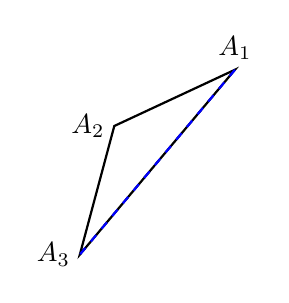
\begin{tikzpicture}[scale=0.8]
    % 1. 定义七边形的7个顶点坐标
    \coordinate (A1) at (90:2.5cm);
    \coordinate (A2) at (140:2.5cm);
    \coordinate (A3) at (190:2.5cm);
    

    % 2. 绘制七边形的外边框
    \draw[thick] (A1) -- (A2) -- (A3) -- cycle;

    % 3. 从顶点 A1 引出所有对角线（虚线表示）
    \draw[dashed, thick, blue] (A1) -- (A3);
    % \draw[dashed, thick, blue] (A1) -- (A4);


    % 4. 标注顶点名称
    \node[above] at (A1) {$A_1$};
    \node[left] at (A2) {$A_2$};
    \node[left] at (A3) {$A_3$};


  
\end{tikzpicture}
\begin{tikzpicture}[scale=1]
    % 1. 定义七边形的7个顶点坐标
    \coordinate (A1) at (90:2.5cm);
    \coordinate (A2) at (140:2.5cm);
    \coordinate (A3) at (190:2.5cm);
    \coordinate (A4) at (240:2.5cm);
 

    % 2. 绘制七边形的外边框
    \draw[thick] (A1) -- (A2) -- (A3) -- (A4) -- cycle;

    % 3. 从顶点 A1 引出所有对角线（虚线表示）
    \draw[dashed, thick, blue] (A1) -- (A3);
    \draw[dashed, thick, blue] (A1) -- (A4);


    % 4. 标注顶点名称
    \node[above] at (A1) {$A_1$};
    \node[left] at (A2) {$A_2$};
    \node[left] at (A3) {$A_3$};
    \node[below left] at (A4) {$A_4$};
  % 5. 在图形下方添加推导公式说明
    \node[below=1cm, align=center, font=\large] at (A4) {
        $n=4$ 边形，\\从一个顶点\\引出 $(n-3)=1$ 条对角线 \\
        分割成 $(n-2)=2$ 个三角形
    };

 
\end{tikzpicture}
\begin{tikzpicture}[scale=1]
    % 1. 定义七边形的7个顶点坐标
    \coordinate (A1) at (90:2.5cm);
    \coordinate (A2) at (140:2.5cm);
    \coordinate (A3) at (190:2.5cm);
    \coordinate (A4) at (240:2.5cm);
    \coordinate (A5) at (290:2.5cm);


    % 2. 绘制七边形的外边框
    \draw[thick] (A1) -- (A2) -- (A3) -- (A4) -- (A5) --  cycle;

    % 3. 从顶点 A1 引出所有对角线（虚线表示）
    \draw[dashed, thick, blue] (A1) -- (A3);
    \draw[dashed, thick, blue] (A1) -- (A4);


    % 4. 标注顶点名称
    \node[above] at (A1) {$A_1$};
    \node[left] at (A2) {$A_2$};
    \node[left] at (A3) {$A_3$};
    \node[below left] at (A4) {$A_4$};
    \node[below right] at (A5) {$A_5$};
  % 5. 在图形下方添加推导公式说明
    \node[below=1cm, align=center, font=\large] at (A5) {
        $n=5$ 边形，\\从一个顶点\\引出 $(n-3)=2$ 条对角线 \\
        分割成 $(n-2)=3$ 个三角形
    };

  
\end{tikzpicture}
\begin{tikzpicture}[scale=1.2]
    % 1. 定义七边形的7个顶点坐标
    \coordinate (A1) at (90:2.5cm);
    \coordinate (A2) at (140:2.5cm);
    \coordinate (A3) at (190:2.5cm);
    \coordinate (A4) at (240:2.5cm);
    \coordinate (A5) at (290:2.5cm);
    \coordinate (A6) at (340:2.5cm);
   

    % 2. 绘制七边形的外边框
    \draw[thick] (A1) -- (A2) -- (A3) -- (A4) -- (A5) -- (A6) --  cycle;

    % 3. 从顶点 A1 引出所有对角线（虚线表示）
    \draw[dashed, thick, blue] (A1) -- (A3);
    \draw[dashed, thick, blue] (A1) -- (A4);
    \draw[dashed, thick, blue] (A1) -- (A5);


    % 4. 标注顶点名称
    \node[above] at (A1) {$A_1$};
    \node[left] at (A2) {$A_2$};
    \node[left] at (A3) {$A_3$};
    \node[below left] at (A4) {$A_4$};
    \node[below right] at (A5) {$A_5$};
    \node[right] at (A6) {$A_6$};


    % 5. 在图形下方添加推导公式说明
    \node[below=1cm, align=center, font=\large] at (A5) {
        $n=6$ 边形，\\从一个顶点引出\\ $(n-3)=3$ 条对角线 \\
        分割成 $(n-2)=4$ 个三角形
    };
\end{tikzpicture}
\begin{tikzpicture}[scale=1.2]
    % 1. 定义七边形的7个顶点坐标
    \coordinate (A1) at (90:2.5cm);
    \coordinate (A2) at (140:2.5cm);
    \coordinate (A3) at (190:2.5cm);
    \coordinate (A4) at (240:2.5cm);
    \coordinate (A5) at (290:2.5cm);
    \coordinate (A6) at (340:2.5cm);
    \coordinate (A7) at (10:2.5cm);

    % 2. 绘制七边形的外边框
    \draw[thick] (A1) -- (A2) -- (A3) -- (A4) -- (A5) -- (A6) -- (A7) -- cycle;

    % 3. 从顶点 A1 引出所有对角线（虚线表示）
    \draw[dashed, thick, blue] (A1) -- (A3);
    \draw[dashed, thick, blue] (A1) -- (A4);
    \draw[dashed, thick, blue] (A1) -- (A5);
    \draw[dashed, thick, blue] (A1) -- (A6);

    % 4. 标注顶点名称
    \node[above] at (A1) {$A_1$};
    \node[left] at (A2) {$A_2$};
    \node[left] at (A3) {$A_3$};
    \node[below left] at (A4) {$A_4$};
    \node[below right] at (A5) {$A_5$};
    \node[right] at (A6) {$A_6$};
    \node[right] at (A7) {$A_7$};

    % 5. 在图形下方添加推导公式说明
    \node[below=1cm, align=center, font=\large] at (A5) {
        $n=7$ 边形\\，从一个顶点引出\\ $(n-3)=4$ 条对角线 \\
        分割成 $(n-2)=5$ 个三角形
    };
\end{tikzpicture}
\subsection*{证明思路：化多边形为三角形}
我们知道三角形的内角和是 $180^\circ$。如果能把一个 $n$ 边形分割成若干个互不重叠的三角形，那么这些三角形的内角和的总和，就等于该多边形的内角和。

\subsection*{证明过程}

\textbf{第 1 步：观察特例}
\begin{itemize}
    \item \textbf{四边形 ($n=4$)：} 从一个顶点出发，可以引出 $1$ 条对角线，将四边形分割成 $2$ 个三角形。\\
    内角和 $= 2 \times 180^\circ = (4-2) \times 180^\circ$。
    \item \textbf{五边形 ($n=5$)：} 从一个顶点出发，可以引出 $2$ 条对角线，将五边形分割成 $3$ 个三角形。\\
    内角和 $= 3 \times 180^\circ = (5-2) \times 180^\circ$。
    \item \textbf{六边形 ($n=6$)：} 从一个顶点出发，可以引出 $3$ 条对角线，将六边形分割成 $4$ 个三角形。\\
    内角和 $= 4 \times 180^\circ = (6-2) \times 180^\circ$。
\end{itemize}

\textbf{第 2 步：推广到 $n$ 边形}
对于任意的 $n$ 边形（$n \ge 3$），我们任选其中一个顶点 $A$：
\begin{enumerate}
    \item 顶点 $A$ 本身不能与自己连线。
    \item 顶点 $A$ 与它相邻的两个顶点连线是多边形的边，不是对角线。
    \item 因此，从顶点 $A$ 出发，可以向除了自身和相邻两点之外的其余顶点引对角线。
\end{enumerate}

所以，从一个顶点出发，一共可以引出 \textbf{$(n-3)$} 条对角线。

\textbf{第 3 步：计算三角形个数与内角和}
这 $(n-3)$ 条对角线，将整个 $n$ 边形分割成了 \textbf{$(n-2)$} 个三角形。
因为这些三角形的所有内角恰好拼成了 $n$ 边形的所有内角，所以：
\[
n \text{ 边形的内角和} = \text{三角形个数} \times 180^\circ
\]
\[
\text{即：} \quad \text{内角和} = (n-2) \times 180^\circ
\]

\subsection*{结论}
通过上述推导，我们证明了任意 $n$ 边形的内角和公式为：
\[
\boxed{(n-2) \times 180^\circ}
\]
\end{document}